%%评价flow direction，挑选出10 valuable flow direction，形式从port_begin到port_end
\section{Task1: Flow Direction Selection}
In this part, we want to filter out ten flow directions with sample value for the pricing system we designed. Because there are contract markets and spot markets in the shipping market, the two influence each other. Our research object is ordinary commodities in the spot market, so we will screen based on the entire market and continue our research.

\subsection {Construct Evaluation System}
We have the following thoughts on the evaluation system for screening flow directions. Since they are used for system testing, they should meet the large number and diversity of samples. Additionally, the ten flow directions should have wealth potential. Therefore, we build an evaluation system as shown in the figure \ref{fig:layer of evaluation}. By using sales volume to reflect the sample size of the flow direction, historical revenue and freight rates to map its wealth potential, and throughput to incarnate its diversity.
\begin{figure}[H]
    \centering
    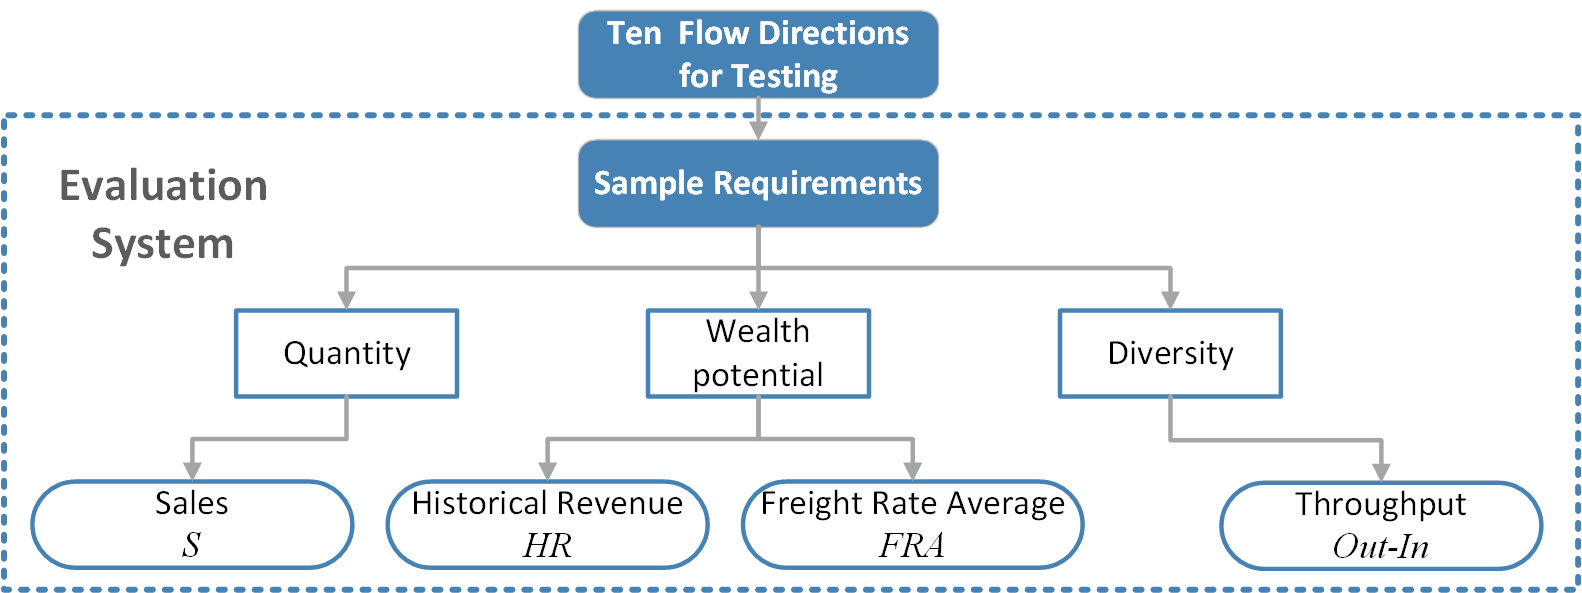
\includegraphics[scale=0.5]{Chapter-Mock/images-Mock/evaluation .png}
    \caption{Evaluation System Structure.}
    \label{fig:layer of evaluation}
\end{figure}

\subsection{Data Processing and Criteria Forming}
The given data set includes 9 properties of the transaction: the ID of one container, the container type, the number of one waybill, the transaction time of one waybill, names of goods, SVVD, AMT (the freight rate), the departure port of the container and the arrival port of the container. In all these properties, we only retain data with containers that are 20 units to simplify the model. And observing these data we find that the freight rate is the same for different goods in the same SVVD at the same time. So we delete the Names of goods and transaction time which are also useless for our evaluation. Then we can obtain the parameters we need according to the following formula definition. 
\begin{itemize}              
    \item Sales ($S$) is the number of waybills. We define the number of container orders as $order\_{quantity}$ (equivalent to sales volume) and the number of times the same waybill is repeated is $repeated\_{counting}$. So we get the formula：
        \begin{equation*}
            S = order\_{quantity} - repeated\_{counting}
        \end{equation*}
   It is noticed that one waybill may include more than one container, so we should delete the repeated counting.
    \item Historical Revenue($HR$) is the sum of the freight rate corresponding to each container, assuming there are $n$ containers in total.
        \begin{equation*}
            HR = \sum_{i=1}^n fr_i
        \end{equation*}
    \item Average Freight Rate($AFR$) is the total revenue divided by the number of orders.
        \begin{equation*}
            AFR = \sum_{i=1}^n fr_i / order\_{quantity}
        \end{equation*}
    \item Port throughput is an important quantitative indicator that reflects the results of port production and operation activities.We define the throughput of the departure port as $Departure_{Ability}$ and the throughput at the arrival port as $Arrival_{Ability}$.The variety of flow directions is directly proportional to both.So We take the average of $Departure_{Ability}$ and $Arrival_{Ability}$ to get $Out\_{in}$ to reflect the throughput.
        \begin{equation*}
            Out\_{in} = \frac{1}{2} (Departure_{Ability} + Arrival_{Ability})
        \end{equation*}
   
\end{itemize}

\subsection{Flow Direction Evaluation}
Following the criteria forming, we will analyze which ten flow directions turns out to be the most valuable ones. In our work, we have designated four criteria based on the data set. The criteria include: HR (Historical Revenue), SV (Sales Volume), AFR (Average Freight Rate), and RA (Region Ability). 

\begin{table}[H]
    \renewcommand\arraystretch{2}   %%控制行间距
    \centering
    \caption{Criteria for Evaluating Flow Direction.}
    \begin{tabular}{cc}    %%三列均左对齐
        \toprule  %%表格横线加粗
        \specialrule{0em}{2pt}{2pt}    %%添加透明线控制行高
        Criteria & Entropy Weight \\
        \specialrule{0em}{2pt}{2pt}    %%添加透明线控制行高
        \midrule
        \specialrule{0em}{1pt}{1pt}
        $HR$ & 0.136367 \\
        $SV$ & 0.652110 \\
        $AFR$ & 0.038062 \\
        $Out\_{in}$ & 0.173461 \\
        \specialrule{0em}{1pt}{1pt}
        \bottomrule
    \label{tbl:Mock-Criteria for Evaluating Flow Direction.}
    \end{tabular}
\end{table}
\vspace{-1cm}

Judging the most valuable flow direction requires melting the above four criteria into a synthetic one. Here we apply \textbf{Entropy Weight Method} to allocate weights to each criterion, and the results are presented in the Table \ref{tbl:Mock-Criteria for Evaluating Flow Direction.}. After that, we utilize \textbf{TOPSIS} (Technique for Order Preference by Similarity to an Ideal Solution) to score each flow direction to filter out the ten flow directions with the highest scores.

\begin{table}[H]
    \renewcommand\arraystretch{2}   %%控制行间距
    \centering
    \caption{TOPSIS Evaluation Results.}
    \begin{tabular}{ccc}    %%三列均左对齐
        \toprule  %%表格横线加粗
        \specialrule{0em}{2pt}{2pt}    %%添加透明线控制行高
        Departure Port & Arrival Port & Score \\
        \specialrule{0em}{2pt}{2pt}    %%添加透明线控制行高
        \midrule
        \specialrule{0em}{1pt}{1pt}
        Yingkou & Ningbo & 0.003902 \\
        Xingang & Nansha & 0.003591 \\
        Yingkou & Nansha & 0.003588 \\
        Yingkou & Fuqing & 0.002518 \\
        Yingkou & Qinzhou & 0.002301 \\
        Yingkou & Shenzhen (Dachan Bay) & 0.001892 \\
        Yingkou & Shantou & 0.001799 \\
        Quanzhou & Yingkou & 0.001709 \\
        Lecong & Yingkou & 0.001592 \\
        Yingkou & Haikou & 0.001574 \\
        \specialrule{0em}{1pt}{1pt}
        \bottomrule
    \label{tbl:Mock-TOPSIS Evaluation Results.}
    \end{tabular}
\end{table}
To conclude, the ten most valuable flow directions are listed in the above table (see in Table \ref{tbl:Mock-TOPSIS Evaluation Results.}) according to the scores by TOPSIS evaluation. Then we mark the departure and arrival ports on the map, complete the direction and finally get the picture of ten flow directions (see in Figure \ref{fig:Mock-flow directions}).
\begin{figure}[H]
    \centering
    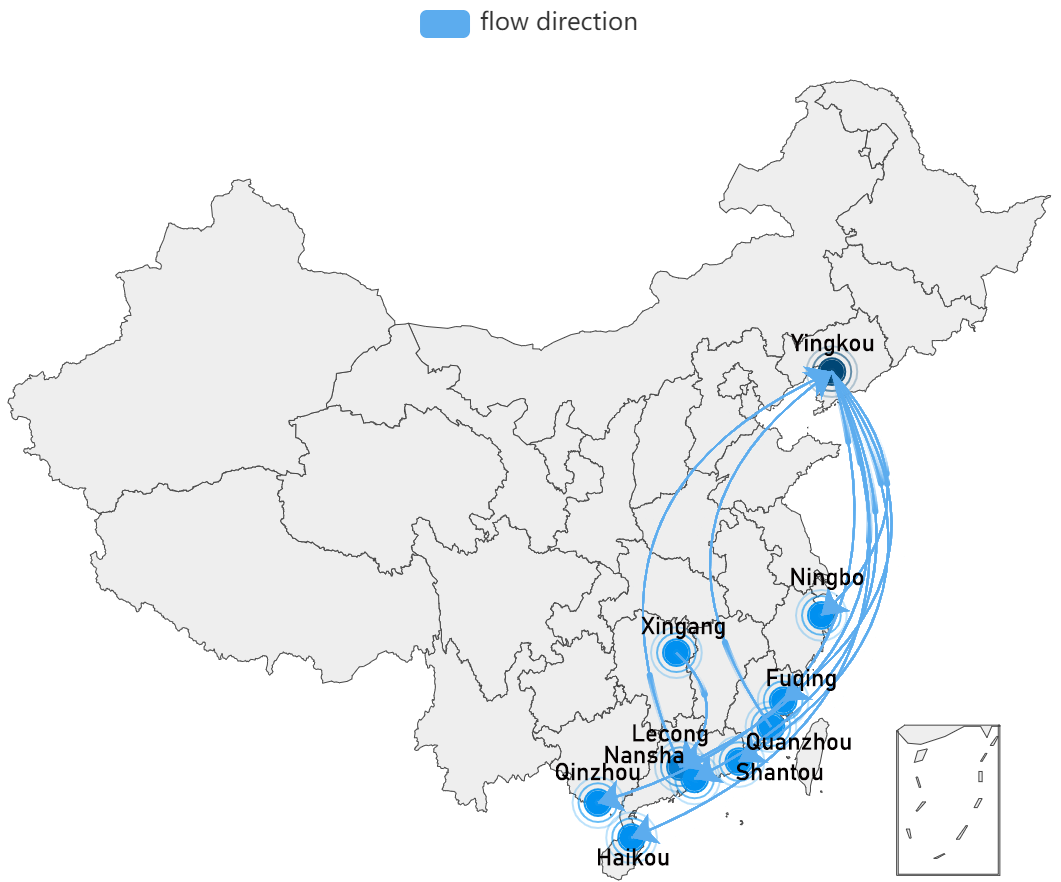
\includegraphics[scale=0.3]{Chapter-Mock/images-Mock/flow directions.png}
    \caption{Flow Directions.}
    \label{fig:Mock-flow directions}
\end{figure}

It can be seen from the table and the figure that almost all ten flow directions contain the city Yingkou, seven in departure ports and two in arrival ports. We believe that coastal routes occupy the main route sample because of its high transaction volume and large value. At the same time, it also contains an inland route, maintaining the diversity of the samples.So far, ten most valuable sample flow directions have been selected.

